% ### by András Kiss ###
% ### 2018.06.20 #######
% ### Homburg ##########


\documentclass[a4paper, 11pt]{article}
\usepackage{ae,aecompl}
\usepackage[T1]{fontenc}
\usepackage[utf8]{inputenc}
\usepackage{indentfirst}
\usepackage{xymtex}
\usepackage{multirow}
\usepackage{gensymb}
\usepackage{upgreek}
\usepackage[geometry]{ifsym}
\usepackage{subfig}
\usepackage[version=3]{mhchem}
\usepackage{float}
\usepackage{textcomp}
\frenchspacing
\usepackage[dvips]{graphicx}
\usepackage{color}
\usepackage{anysize}
\marginsize{3.2cm}{2.8cm}{3cm}{2cm}
\usepackage{enumerate}
\usepackage{cite}
\usepackage{listings}
\usepackage{setspace}
\setstretch{1.2}
\usepackage{xcolor}
\usepackage{listings}
% uncomment for hyperlinks
\usepackage[colorlinks = true,
            linkcolor = red,
            urlcolor  = blue,
            citecolor = blue,
            anchorcolor = blue]{hyperref}

\begin{document}
\thispagestyle{empty}

%\begin{figure}
%\centering
%\includegraphics[width=0.45\textwidth, angle=-90]{11.eps}
%\includegraphics[width=0.45\textwidth, angle=-90]{11_deconvoluted.eps}
%\includegraphics[width=0.45\textwidth, angle=-90]{11_wiener_deconvoluted.eps}
%\caption{(A) Original raw image of the human monocyte. (B) After temporal deconvolution. (C) After temporal and spatial deconvolution. The Wiener--algorithm was used assuming a perfect d = 10 $\upmu$m Pt disk UME. Noise in the last step increased significantly. Circles in the lower right corner show the size of the electrode. Tip potential was 650 mV against a quasi-reference Ag/AgCl electrode. The UME was oxidizing H$_2$O$_2$.}
%\label{fig:results}
%\end{figure}

\thispagestyle{empty}
\begin{figure}
\centering
\includegraphics[width=0.45\textwidth, angle=-90]{140514/6_original.eps}
\includegraphics[width=0.45\textwidth, angle=-90]{140514/6_deconvoluted.eps}
\caption{}
\label{fig:results}
\end{figure}




\end{document}

